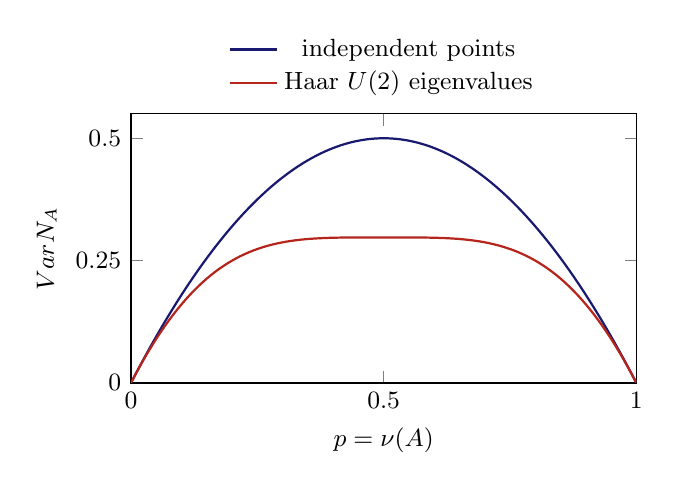
\begin{tikzpicture}
\begin{axis}[width=8cm,height=5cm,xmin=0,xmax=1,ymin=0,ymax=.55,
 xlabel={$p=\nu(A)$},ylabel={$\operatorname{Var}N_A$},
 xtick={0,.5,1},ytick={0,.25,.5},
 legend style={at={(.5,1.03)},anchor=south,draw=none,font=\small},
 tick label style={font=\small},label style={font=\small}]
\addplot[MidnightBlue,thick,domain=0:1,samples=121]{2*x*(1-x)};
\addlegendentry{independent points}
\addplot[BrickRed,thick,domain=0:1,samples=121]{2*x-2*x*x-2*(sin(deg(pi*x))/pi)^2};
\addlegendentry{Haar $U(2)$ eigenvalues}
\end{axis}
\end{tikzpicture}
